\chapter{数学基础知识}
\label{chap:math basics}

\section{线性空间}
\label{sec:linear space}

\subsection{线性空间}

\begin{definition}
    {线性空间}{linear space}
    给定一个数域$\FF$ (本笔记只涉及实数域$\RR$和复数域$\CC$)和一个集合$V$,
    
    定义加法$+:V\times V\to V$满足:
    \begin{itemize}
        \item 结合律:$(a+b)+c=a+(b+c),$
        \item 零元:$a+0=a,$
        \item 逆元:$a+(-a)=0,$
        \item 交换律:$a+b=b+a;$
    \end{itemize}
    数乘$\cdot:\FF\times V\to V$满足:
    \begin{itemize}
        \item 单位元:$1a=a,$
        \item 结合律:$(\lambda\mu)a=\lambda(\mu a),$
        \item 分配率1:$(\lambda+\mu)a=\lambda a+\mu a,$
        \item 分配率2:$\lambda(a+b)=\lambda a+\lambda b.$
    \end{itemize}
    则称$V$在$\FF$上构成一个线性空间(linear space)。
\end{definition}

\begin{example}
    {线性空间的例子}{}
    \begin{itemize}
        \item $\cont^n[a,b]$:全体在$[a,b]$上$n$次导数连续(continuous)的函数构成的集合。
        % \item $\diff^n[a,b]$:全体在$[a,b]$上$n$次可导(differentiable)的函数构成的集合。
        \item $\poly_n=\set{a_0+a_1x+\cdots+a_nx^n}{a_i\in\FF}$:$n$次多项式函数空间。
        % \item 正实数$\RR_{>0}$构成一个线性空间,其加法为实数乘法,数乘为幂次。
    \end{itemize}
\end{example}

\subsection{线性空间的基和维度}

\begin{definition}
    {线性无关}{linear independent}
    设$V$是线性空间,给定其中$n$个元素$x_1,\ldots,x_n\in V$,若%其线性组合(linear combination)
    \begin{equation}
        a_1x_1+\cdots+a_nx_n=0,\iff a_1=\cdots=a_n=0,
    \end{equation}
    则称$x_1,\ldots,x_n$线性无关(linear independent)。反之,称为线性相关。
\end{definition}

\begin{example}
    {线性无关的例子}{}
    \begin{itemize}
        \item $\poly_n$中$\{1,x,\ldots,x^n\}$是线性无关的;
        \item 所有$[-\pi,\pi]$上的周期函数构成的函数空间是线性空间,其中
        \[
            \{1,\cos x,\sin x,\ldots,\cos nx,\sin nx\} 
        \]
        线性无关。
    \end{itemize}
\end{example}

\begin{definition}
    {线性空间的基和维度}{dimension, base}
    给定线性空间$V$中的一组元素$\{x_1,\ldots,x_n\}$,若$\forall x\in V$都可以被唯一表示为其线性组合
    \begin{equation}
        x=a_1x_1+\cdots+a_nx_n,
    \end{equation}
    则称$\{x_1,\ldots,x_n\}$构成一组基(base),且$V$的维度$\dim(V)=n$。
\end{definition}

\begin{theorem}
    {}{}
    线性空间的维度与基的选取没有关系。
\end{theorem}

\begin{example}
    {典型线性空间的维度}{}
    \begin{itemize}
        \item $\dim(\poly_n)=n;$
        \item $\dim(\cont[a,b])=+\infty.$
    \end{itemize}
\end{example}

\section{范数}
\label{sec:norm}

\subsection{度量空间}

\begin{definition}
    {度量空间}{metric space}
    给定集合$M$,若映射$d:M\times M\to\RR$满足:
    \begin{itemize}
        \item 正定性:$d(x,y)\geq 0$,且$d(x,y)=0\iff x=y$;
        \item 交换性:$d(x,y)=d(y,x)$;
        \item 三角不等式:$d(x,y)+d(y,z)\geq d(x,z)$。
    \end{itemize}
    则称$M$是一个度量空间(metric space)或距离空间,$d$为度量函数或距离函数。
\end{definition}

\begin{definition}
    {Cauchy序列}{Cauchy sequence}
    对于序列$\{x_n\}$,若$\forall\varepsilon>0,\exists N\in\NN$满足:
    \begin{equation}
        d(x_m,x_n)<\varepsilon,\quad\forall m,n>N,
    \end{equation}
    则称$\{x_n\}$为Cauchy序列(Cauchy sequence)。
\end{definition}

\begin{definition}
    {度量空间的完备性}{completeness}
    若$\forall$ Cauchy序列$\{x_n\}\subset M$,$\exists x\in M$满足:
    \[
        \lim_{n\to\infty}d(x_n,x)=0,\iff\lim_{n\to\infty}x_n=x,
    \]
    则称度量空间$M$是完备的(complete)。
\end{definition}

\begin{remark}
    不严谨地说,完备性要求:所有收敛的序列都会收敛到$M$中。%即$M$中没有“缺失点”。
\end{remark}

\begin{example}
    {实数公理}{}
    实数集$\RR$中的度量函数$d(a,b)=|a-b|$是完备的。
\end{example}

\begin{theorem}
    {完备化定理}{}
    若$(M,d)$是一个度量空间,则存在唯一等距同构的完备化空间。%一个从$M$到一个完备度量空间的等距嵌入。
\end{theorem}

\begin{proof}
    构造性证明,令$\tilde M$是$M$中所有Cauchy序列$\{x_n\}$的集合。在$\tilde M$中定义等价关系$\sim$:
    \[
        \{x_n\}\sim\{y_n\}\iff\lim_{n\to\infty}d(x_n,y_n)=0.
    \]
    令$[\{x_n\}]=\nset{\{y_n\}}{\{x_n\}\sim\{y_n\}}$表示$\{x_n\}$的等价类,$\hat M=\nset{[\{x_n\}]}{\{x_n\}\in\tilde M}$是$M$中所有Cauchy序列的等价类构成的集合。定义$\hat M$上的度量为
    \[
        \hat d([\{x_n\}],[\{y_n\}]):=\lim_{n\to\infty}d(x_n,y_n),
    \]
    可证$(\hat M,\hat d)$是完备的度量空间。且存在等距嵌入
    \[
        i:M\to\hat M,\enspace x\mapsto[\{x,x,\ldots\}].
    \]
    即$i$是映射到对应常数序列的等价类。
\end{proof}

\subsection{赋范空间与范数}

\begin{definition}
    {赋范空间与范数}{normed space}
    若映射$\norm\cdot:S\to\RR$满足:
    \begin{itemize}
        \item 正定性:$\norm f\geq 0$,且$\norm f=0\iff f=0$;
        \item 齐次性:$\norm{\lambda f}=\abs\lambda\norm f$;
        \item 三角不等式:$\norm{f+g}\leq\norm f+\norm g$。
    \end{itemize}
    则称$(S,\norm\cdot)$构成一个赋范空间(normed space),$\norm\cdot$是$S$的范数(norm)。
\end{definition}

\begin{corollary}
    显然,赋范空间也是度量空间,只需定义
    \[
        d(f,g)=\norm{f-g},
    \]
\end{corollary}
\begin{remark}
    赋范空间不一定是完备的,完备的赋范空间也称为Banach空间。
\end{remark}

\begin{example}
    {$\RR^n$的$p$ - 范数}{vector p-norm}
    向量$x=(x_1,\ldots,x_n)\tp\in\FF^n$的$p$ - 范数为
    \begin{equation}
        \label{eqn:p-norm vector}
        \norm x_p=\kh{\sum_{i=1}^n\abs{x_i}^p}^{1/p},
        % =\begin{cases}
        %     \max_{i}\abs{x_i},&p=\infty\\
        %     \sum_{i=1}^n\abs{x_i},&p=1\\
        %     \kh{\sum_{i=1}^n\abs{x_i}^2}^{1/2},&p=2
        % \end{cases}
    \end{equation}
    特别地,$\norm x_\infty=\lim_{p\to\infty}\norm x_p=\max_i\abs{x_i}$。
    \begin{proof}
        记$k=\arg\max_i\abs{x_i}$,$\forall p>0$
        \[
            \abs{x_k}^p\leq\sum_{i=1}^n\abs{x_i}^p\leq n\abs{x_k}^p,
        \]
        两边开$p$次方,并$p\to\infty$,即得$\norm x_\infty=\abs{x_k}.$
    \end{proof}
    \tcblower
    二维位置向量$r=(x,y)\in\RR^2$,方程$\norm r_p=1$在直角坐标中的图像为
    \begin{center}
        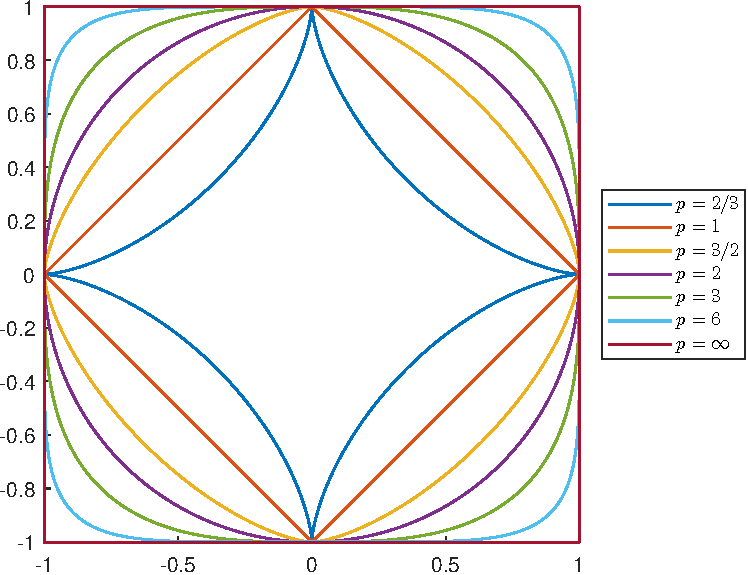
\includegraphics[width=0.6\linewidth]{graphs/Lpspace.pdf}
        \captionof{figure}{不同的$p$ - 范数}
        \label{fig:Lp space}
    \end{center}
    特别地,$p=2/3$的曲线叫星形线(astroid)。
\end{example}

\begin{example}
    {$C[a,b]$的$p$ - 范数}{function p-norm}
    函数$f\in\cont[a,b]$的$p$ - 范数为
    \begin{equation}
        \label{eqn:p-norm function}
        \norm f_p=\kh{\int_a^b\abs{f(x)}^p\d x}^{1/p},
        % =\begin{cases}
        %     \max_{a\leq x\leq b}\abs{f(x)},&p=\infty\\
        %     \int_a^b\abs{f(x)}\d x,&p=1\\
        %     \kh{\int_a^b\abs{f(x)}^2\d x}^{1/2},&p=2
        % \end{cases}
    \end{equation}
    当$1<p<\infty$时,$\norm\cdot_p$是不完备的:连续函数Cauchy序列可以按范数收敛于一个不连续的函数。
    但$\norm\cdot_\infty$是完备的。
\end{example}

\subsection{范数的等价性}

\begin{definition}
    {范数的等价性}{}
    给定线性空间$S$上的两个范数$\norm\cdot_\alpha,\norm\cdot_\beta$,若$\exists C_1,C_2>0$满足:
    \[
        C_1\norm x_\alpha\leq\norm x_\beta\leq C_2\norm x_\alpha,
    \]
    则称$\norm\cdot_\alpha,\norm\cdot_\beta$等价(equivalent)。
\end{definition}

\begin{corollary}
    向量的$p$ - 范数都是等价的,因为由H\"older不等式,$p<q$时
    \begin{equation}
        \norm x_q\leq\norm x_p\leq n^{1/p-1/q}\norm x_p.
    \end{equation}
\end{corollary}

\begin{theorem}
    {}{}
    有限维线性空间中,任意两个范数都是等价的。
\end{theorem}


\section{内积}
\label{sec:inner product}

\begin{definition}
    {内积}{inner product}
    给定线性空间$S$,内积(inner product)是一个映射$\inp\cdot\cdot:S\times S\to\FF$,
    满足:
    \begin{itemize}
        \item 正定性:$\inp xx\geq 0$,且$\inp xx=0\iff x=0;$
        \item 交换共轭:$\inp xy=\overline{\inp yx};$
        \item 对第一个变量线性:$\inp{ax+by}z=a\inp xz+b\inp yz.$
    \end{itemize}
    若$\inp xy=0$,则称$x,y$是正交的(orthogonal)。
\end{definition}

\begin{remark}
    对第二个变量不一定线性,会出现复共轭:
    \[
        \inp x{ay+bz}=\overline a\inp xy+\overline b\inp xz.
    \]
    除非内积的值域$\FF\subset\RR$,此时内积满足对称性:$\inp xy=\inp yx$。
\end{remark}

\begin{corollary}
    根据内积可以自然定义出一个范数,称为内积诱导的范数:
    \begin{equation}
        \norm x:=\sqrt{\inp xx},
    \end{equation}
\end{corollary}

\begin{example}
    {内积实例}{}
    \begin{itemize}
        \item $\CC^n$中的标准内积为
        \[
            \inp xy=\sum_{i=1}^nx_i\overline y_i,
        \]
        标准内积诱导出来的范数就是2 - 范数。
        \item $\cont[a,b]$的一个内积为 
        \[
            \inp fg=\int_a^bf(x)\overline g(x)\d x.
        \]
    \end{itemize}
\end{example}

\begin{definition}
    {Gram矩阵}{Gram matrix}
    给定一组向量$x_1,\ldots,x_n$,Gram矩阵的第$i,j$个元素由内积$\inp{x_i}{x_j}$给出:
    \begin{equation}
        G:=\begin{bmatrix}
            \inp{x_1}{x_1}&\cdots&\inp{x_1}{x_n}\\
            \vdots&\ddots&\vdots\\
            \inp{x_n}{x_1}&\cdots&\inp{x_n}{x_n}
        \end{bmatrix}.
    \end{equation}
\end{definition}

\begin{theorem}
    {内积空间线性无关的判定}{}
    给定内积空间$S$,$x_1,\ldots,x_n\in S$是线性无关的$\iff$ Gram矩阵可逆。
\end{theorem}

\begin{proof}
    设$a=(a_1,\ldots,a_n)$满足$aG=0$,则$\forall k=1,\ldots,n$
    \[
        (aG)_k=a_1\inp{x_1}{x_k}+\cdots+a_n\inp{x_n}{x_k}=\inp{a_1x_1+\cdots,a_nx_n}{x_k}=0,
    \]
    特别地,
    \[
        \inp{a_1x_1+\cdots+a_nx_n}{a_1x_1+\cdots+a_nx_n}=0,\iff a_1x_1+\cdots,a_nx_n=0,
    \]
    则$G$可逆$\iff \mathrm N(G\tp)=\{0\}\iff a$只有零解。
\end{proof}

\begin{example}
    {}{}
    给定内积空间$S$的一组基$\{x_1,\ldots,x_n\}$,则$\forall x\in S$均可以写成
    \[
        x=a_1x_1+\cdots+a_nx_n,
    \]
    下面计算$a_1,\ldots,a_n$。两边分别与$x_i$做内积:
    \[
        \inp x{x_i}=a_1\inp{x_1}{x_i}+\cdots+a_n\inp{x_n}{x_i},
    \]
    即
    \[
        [\inp x{x_1}\enspace\cdots\enspace\inp x{x_n}]=[a_1\enspace\cdots\enspace a_n]G,
    \]
    若基是正交的,即$\forall i\neq j,\enspace\inp{x_i}{x_j}=0$,则 
    \[
        a_i=\frac{\inp x{x_i}}{\inp{x_i}{x_i}}.
    \]
\end{example}

\begin{theorem}
    {Schmidt正交化}{}
    设$x_1,\ldots,x_n$是一组线性无关的基,为得到一组正交基,定义
    \begin{equation}
        y_i=x_i-\sum_{j=1}^{i-1}\frac{\inp{x_i}{y_j}}{\inp{y_j}{y_j}}y_j.
    \end{equation}
    则$y_1,\ldots,y_n$是正交的。
\end{theorem}

\begin{definition}
    {带权内积}{}
    设$\rho\in\cont(a,b)$是一个几乎处处为正\footnote{即$\{x|\rho(x)\leq 0\}$的Lebesgue测度为0。}的函数,且
    \[
        \int_a^b\rho(x)\d x<+\infty,
    \]
    定义内积
    \begin{equation}
        \inp fg=\int_a^bf(x)g(x)\rho(x)\d x.
    \end{equation}
\end{definition}

\begin{definition}
    {正交多项式}{}
    已知$\{1,x,\ldots,x^n\}$是线性无关的。考虑$\cont[a,b]$上的带权内积,Schmidt正交化得到一组多项式函数
    \[
        \psi_0(x),\psi_1(x),\ldots,\psi_n(x),
    \]
    显然,$\deg(\psi_i)=i.$
\end{definition}

\begin{example}
    {Legendre多项式}{Legendre polynomial}
    权函数$\rho=1$,区间$[-1,1]$,得到Legendre多项式
    \begin{equation}
        P_n(x)=\frac1{2^nn!}\dd[n]x(x^2-1)^n.
    \end{equation}
    \begin{itemize}
        \item 内积 
        \begin{equation}
            \inp{P_n}{P_m}=\frac2{2n+1}\delta_{nm}.
        \end{equation}
        \item 递归关系
        \begin{equation}
            (n+1)P_{n+1}(x)=(2n+1)xP_n(x)-nP_{n-1}(x).
        \end{equation}
        \item 奇偶性
        \begin{equation}
            P_n(-x)=(-1)^nP_n(x).
        \end{equation}
    \end{itemize}
\end{example}

\begin{example}
    {Chebyshev多项式}{Chebyshev polynomial}
    权函数$\rho(x)=(1-x^2)^{-1/2}$,区间$[-1,1]$,得到Chebyshev多项式
    \begin{equation}
        T_n(x)=\cos(n\arccos x).
    \end{equation}
    \begin{itemize}
        \item 内积 
        \begin{equation}
            \inp{T_n}{T_n}=\begin{cases}
                \pi,&n=0\\
                \pi/2,&n\geq 1
            \end{cases}
        \end{equation}
        \item 递推关系
        \begin{equation}
            T_{n+1}(x)=2xT_n(x)-T_{n-1}(x).
        \end{equation}
        \item 奇偶性
        \begin{equation}
            T_n(-x)=(-1)^nT_n(x);
        \end{equation}
        \item $T_n$的$n$个实单根为$\cos\biggkh{\frac{2k-1}{2n}\pi}$,$(n+1)$个极值点为$\cos\kh{\frac kn\pi}$
        \item 当$\abs x\geq 1$时,
        \begin{equation}
            T_n(x)=\frac12\fkh{\kh{x+\sqrt{x^2-1}}^k+\kh{x-\sqrt{x^2-1}}^k}.
        \end{equation}
    \end{itemize}
\end{example}

\section{矩阵空间}
\label{sec:matrix space}

\subsection{矩阵范数}

\begin{definition}
    {矩阵范数}{matrix norm}
    矩阵空间上的范数$\norm\cdot:\FF^{n\times n}\to\RR$若满足
    \begin{equation}
        \norm{AB}\leq\norm A\norm B,
    \end{equation}
    则$\norm\cdot$称为矩阵范数(matrix norm)。
\end{definition}

\newcommand{\Forb}[1]{\norm{#1}_{\mathrm F}}


\begin{example}
    {Frobenius范数}{Frobenius norm}
    定义Frobenius范数
    \begin{equation}
        \Forb A:=\sqrt{\sum_{i=1}^n\sum_{j=1}^n\abs{A_{ij}}^2}.
    \end{equation}
    是一个矩阵范数。
    \begin{proof}
        由Cauchy-Schwarz不等式
        \begin{align*}
            \Forb{AB}&=\sqrt{\sum_{i=1}^n\sum_{j=1}^n\abs{\sum_{k=1}^nA_{ik}B_{kj}}^2}\leq\sqrt{\sum_{i=1}^n\sum_{j=1}^n\kh{\sum_{k=1}^n\abs{A_{ik}}^2\sum_{k=1}^n\abs{B_{kj}}^2}}\\
            &=\sqrt{\sum_{i=1}^n\sum_{k=1}^n\abs{A_{ik}}^2\sum_{j=1}^n\sum_{k=1}^n\abs{B_{kj}}^2}=\Forb A\Forb B.
            \qedhere
        \end{align*}
    \end{proof}
    \tcblower
    注意到
    \[
        \tr(A\dg A)=\sum_{i=1}^n(A\dg A)_{ii}=\sum_{i=1}^n\sum_{j=1}^nA\dg_{ij}A_{ji}=\sum_{i=1}^n\sum_{j=1}^n\abs{A_{ji}}^2.
    \]
    故
    \begin{equation}
        \Forb A=\sqrt{\tr(A\dg A)}=\sqrt{\tr(AA\dg)}.
    \end{equation}
\end{example}

\begin{definition}
    {矩阵范数与向量范数的相容}{}
    给定矩阵范数$\norm\cdot_M$和向量范数$\norm\cdot_V$,若$\forall A\in\FF^{n\times n},x\in\FF^n$ 
    \begin{equation}
        \norm{Ax}_V\leq\norm A_M\norm x_V,
    \end{equation}
    则称他们是相容的。在不引起混淆的情况下,可以略去下标。
\end{definition}

\begin{theorem}
    {}{}
    Frobenius范数与向量2 - 范数相容。
\end{theorem}

\begin{proof}
    \[
        \norm{Ax}_2=\sqrt{\sum_{i=1}^n\abs{\sum_{j=1}^n A_{ij}x_j}^2}\leq\sqrt{\sum_{i=1}^n\kh{\sum_{j=1}^n\abs{A_{ij}}^2\sum_{j=1}^n\abs{x_j}^2}}=\Forb A\norm x_2.
        \qedhere
    \]
\end{proof}

\subsection{算子范数}

\begin{definition}
    {算子范数}{operate norm}
    定义矩阵的算子范数(operate norm)
    \begin{equation}
        N:\FF^{n\times n}\to\RR,\enspace A\mapsto\sup_{x\neq 0}\frac{\norm{Ax}}{\norm x}.
    \end{equation}
    称算子范数是该向量范数诱导出来的矩阵范数。
\end{definition}

\begin{remark}
    注意$N(I)=1$。故Frobenius范数不是算子范数。
\end{remark}

\begin{theorem}
    {}{}
    $N(\cdot)$是一个矩阵范数,并与向量范数相容。 
\end{theorem}

\begin{proof}
    % 若$N(A)=0$,则$\forall x,Ax=0$,于是$A=0$;否则
    易得$\forall x\neq 0,\enspace\norm{Ax}\leq N(A)\norm x$。
    \[
        N(AB)=\sup_{x\neq 0}\frac{\norm{ABx}}{\norm x}\leq\sup_{x\neq 0}\frac{N(A)\norm{Bx}}{\norm x}=N(A)N(B).
        \qedhere
    \]
\end{proof}

\begin{definition}
    {谱半径}{spectrum}
    矩阵$A$全体特征值的集合称为$A$的谱(spectrum),记作$\sigma(A)$,特征值模的最大值称为谱半径,记作$\rho(A)$。
\end{definition}

\begin{remark}
    对于一般的矩阵$A\in\FF^{m\times n}$,有$\sigma(A\dg A)\cup\{0\}=\sigma(AA\dg)\cup\{0\}$,即非0特征值相同,其元素称为$A$的奇异值(sigular value)。
\end{remark}

\begin{example}
    {}{}
    设$A\in\FF^{n\times n}$,则$p$ - 向量范数诱导出来的矩阵范数为:
    \begin{subequations}
        \label{eqn:op norm}
        \begin{align}
            \label{eqn:op inf-norm}
            \norm A_\infty&=\max_{i}\sum_{j=1}^n\abs{A_{ij}},\\
            \label{eqn:op 1-norm}
            \norm A_1&=\max_{j}\sum_{i=1}^n\abs{A_{ij}},\\
            \label{eqn:op 2-norm}
            \norm A_2&=\sqrt{\rho(A\dg A)},
        \end{align}
    \end{subequations}
    \begin{proof}
        先证明\eqref{eqn:op 1-norm},将$A$写作列向量的形式$(A_1,\ldots,A_n)$,令$k=\arg\max_j\norm{A_j}_1$,则$\forall x\in\FF^n$且$\norm x_1=\sum_{j=1}^n\abs{x_j}=1$,有
        \[
            \norm{Ax}_1=\norm{\sum_{j=1}^nA_jx_j}_1\leq\sum_{j=1}^n\abs{x_j}\norm{A_j}_1\leq\norm{A_k}_1\sum_{j=1}^n\abs{x_j}=\norm{A_k}_1\norm x_1=\norm{A_k}_1,
        \]
        特别地,取$x=e_k$可使等号成立,故
        \[
            \norm A_1=\sup_{\norm x_1=1}\norm{Ax}_1=\norm{A_k}_1=\max_{j}\sum_{i=1}^n\abs{A_{ij}};
        \]
        然后证明\eqref{eqn:op inf-norm},令$k=\arg\max_i\sum_{j=1}^n\abs{A_{ij}}$,$\forall x\in\FF^n$且$\norm x_\infty=\max_j\abs{x_j}=1$,有
        \[
            \norm{Ax}_\infty=\max_i\abs{\sum_{j=1}^nA_{ij}x_j}\leq\max_i\sum_{j=1}^n\abs{A_{ij}}\abs{x_j}\leq\max_i\sum_{j=1}^n\abs{A_{ij}}\max_j\abs{x_j}=\sum_{j=1}^n\abs{A_{kj}}.
        \]
        特别地,取$x_j=\sgn(A_{kj})$可使等号成立,故 
        \[
            \norm A_\infty=\sup_{\norm x_\infty=1}\norm{Ax}_\infty=\max_i\sum_{j=1}^n\abs{A_{ij}};
        \]
        最后证明\eqref{eqn:op 2-norm},由2 - 范数的性质:
        \[
            \norm A_2^2=\sup_{\norm x_2=1}\inp{Ax}{Ax}=\sup_{\norm x_2=1}\inp{A\dg Ax}{x}=\rho(A\dg A).
            \qedhere
        \]
    \end{proof}
\end{example}

\begin{theorem}
    {谱半径小于矩阵范数}{rho<=norm}
    谱半径$\rho(A)$和矩阵范数的关系:
    \begin{equation}
        \rho(A)\leq\norm A.
    \end{equation}
\end{theorem}

\begin{proof}
    考虑$A$的一个特征值$\lambda$和特征向量$x$,则 
    \[
        \abs\lambda\norm{xx'}=\norm{Axx'}\leq\norm A\norm{xx'}.
    \]
    于是$\norm A\geq\abs\lambda$。
\end{proof}

\begin{theorem}
    {}{norm<=rho+eps}
    给定$A\in\FF^{n\times n},\epsilon>0$,存在算子范数$\norm\cdot$满足:
    \begin{equation}
        \norm A\leq\rho(A)+\epsilon.
    \end{equation}
\end{theorem}

\begin{lemma}
    若$\norm\cdot_\alpha$是$\FF^n$中的向量范数,$P\in\FF^{n\times n}$非奇异,则
    \[
        \norm\cdot_{P,\alpha}:x\mapsto\norm{Px}_\alpha,
    \]
    构成另一个向量范数,诱导的算子范数为
    \[
        \norm{A}_{P,\alpha}=\nnorm{PAP\iv}_\alpha.
    \]
\end{lemma}

\begin{proof}
    令$P$将$A$相似变换为Jordan型,即
    \[
        PAP\iv=J=\diag(J_1,\ldots,J_r),\quad J_i=\begin{bmatrix}
            \lambda_i&1\\
            &\ddots&\ddots\\
            &&\ddots&1\\
            &&&\lambda_i
        \end{bmatrix}
    \]
    令$D_\epsilon=\diag(1,\epsilon,\ldots,\epsilon^{n-1})$,则 
    \[
        \hat J=D_\epsilon\iv JD_\epsilon=\diag(\hat J_1,\ldots,\hat J_r),\quad\hat J_i=\begin{bmatrix}
            \lambda_i&\epsilon\\
            &\ddots&\ddots\\
            &&\ddots&\epsilon\\
            &&&\lambda_i
        \end{bmatrix}
    \]
    则
    \[
        \norm A_{D_\epsilon\iv P,\infty}=\nnorm{D_\epsilon\iv PAP\iv D_\epsilon}_\infty=\nnorm{\hat J}_\infty\leq\rho(A)+\epsilon.
        \qedhere
    \]
\end{proof}

\begin{remark}
    对任意满足$\abs\lambda=\rho(A)$的特征值$\lambda$,对应Jordan块是对角的,则存在一个算子范数满足
    \[
        \norm A=\rho(A).
    \]
\end{remark}

\subsection{扰动定理}

一个矩阵不可逆的概率是很低的,\footnote{因为多了一个$\det(A)=0$的限制条件。}那如何度量矩阵的奇异性?%用逆的大小。

\begin{theorem}
    {扰动定理}{perturbation theorem I}
    给定扰动$B$,若$\norm B<1$,则$I+B$可逆且
    \begin{equation}
        \nnorm{(I+B)\iv}\leq\frac1{1-\norm B}.
    \end{equation}
\end{theorem}

\begin{proof}
    若$I+B$不可逆,则$\rho(B)\geq 1>\norm B$矛盾。
    记$D:=(I+B)\iv$,则 
    \[
        (I+B)D=I,\iff D=I-BD,\implies \norm D\leq 1+\norm B\norm D.
        \qedhere
    \]
\end{proof}

\begin{theorem}
    {扰动定理·二}{perturbation theorem II}
    给定$A,C$,若$A$非奇异且
    \[
        \norm{C-A}\leq\nnorm{A\iv}\iv,
    \]
    则$C$也非奇异,且
    \begin{equation}
        \norm{C\iv}\leq\frac{1}{\nnorm{A\iv}\iv-\norm{C-A}}.
    \end{equation}
\end{theorem}

\begin{proof}
    令$B=I-A\iv C$即可。
\end{proof}



